%%%%%%%%%%%%%%%%%%%%%%%%%%%%%%%%%%%%%%%%%
% Stylish Article
% LaTeX Template
% Version 2.1 (1/10/15)
%
% This template has been downloaded from:
% http://www.LaTeXTemplates.com
%
% Original author:
% Mathias Legrand (legrand.mathias@gmail.com) 
% With extensive modifications by:
% Vel (vel@latextemplates.com)
%
% License:
% CC BY-NC-SA 3.0 (http://creativecommons.org/licenses/by-nc-sa/3.0/)
%
%%%%%%%%%%%%%%%%%%%%%%%%%%%%%%%%%%%%%%%%%

%----------------------------------------------------------------------------------------
%	PACKAGES AND OTHER DOCUMENT CONFIGURATIONS
%----------------------------------------------------------------------------------------

\documentclass[fleqn,10pt]{SelfArx} % Document font size and equations flushed left

\usepackage[english]{babel} % Specify a different language here - english by default

\graphicspath{ {./img/} }

\usepackage{float}

\usepackage[export]{adjustbox}

%----------------------------------------------------------------------------------------
%	COLUMNS
%----------------------------------------------------------------------------------------

\setlength{\columnsep}{0.55cm} % Distance between the two columns of text
\setlength{\fboxrule}{0.75pt} % Width of the border around the abstract

%----------------------------------------------------------------------------------------
%	COLORS
%----------------------------------------------------------------------------------------

\definecolor{color1}{RGB}{0,0,90} % Color of the article title and sections
\definecolor{color2}{RGB}{200,200,200} % Color of the boxes behind the abstract and headings
\definecolor{color3}{RGB}{200,200,200}

%----------------------------------------------------------------------------------------
%	HYPERLINKS
%----------------------------------------------------------------------------------------

\usepackage{hyperref} % Required for hyperlinks
\hypersetup{hidelinks,colorlinks,breaklinks=true,urlcolor=color1,citecolor=color1,linkcolor=color1,bookmarksopen=false,pdftitle={Title},pdfauthor={Author}}

%----------------------------------------------------------------------------------------
%	ARTICLE INFORMATION
%----------------------------------------------------------------------------------------

\JournalInfo{Introduction to Data Analysis  and Mining 2022} % Journal information
\Archive{} % Additional notes (e.g. copyright, DOI, review/research article)

\PaperTitle{Semester Project} % Article title

\Authors{Joshua Elms\textsuperscript{1}*} % Authors
\affiliation{\textsuperscript{1}\textit{Data Science, School of Informatics , Computing and Engineering, Indiana University, Bloomington, IN, USA}} % Author affiliation


\Keywords{Meteorology --- Numerical Weather Prediction --- Machine Learning} % Keywords - if you don't want any simply remove all the text between the curly brackets
\newcommand{\keywordname}{Keywords} % Defines the keywords heading name

%----------------------------------------------------------------------------------------
%	ABSTRACT
%----------------------------------------------------------------------------------------

\Abstract{This data analytics project is focused on predicting the size of largest hailstone that comes from any given storm. To do this, reports of more than 20,000 hail events and their associated meteorological data have been collected and tabularized.}

%----------------------------------------------------------------------------------------

\begin{document}

\flushbottom % Makes all text pages the same height

\maketitle % Print the title and abstract box

\tableofcontents % Print the contents section

\thispagestyle{empty} % Removes page numbering from the first page




%----------------------------------------------------------------------------------------
%Problem and Data Description
%----------------------------------------------------------------------------------------


\section{Problem and Data Description} % The \section*{} command stops section numbering

According to the NOAA Annual Severe Weather website, there were 3,762 recorded severe hail events (hail over 0.75") in the US in 2021 alone. Beyond the noble goal of furthering our understanding of the natural world, the ability to accurately predict which locations will experience hail storms could benefit insurance companies who \href{https://www.insurance.com/coverage/home-hail-damage-insurance-claims#:~:text=hail\%20damage\%20insurance-,Average\%20insurance\%20payout\%20for\%20hail\%20damage,may\%20be\%20higher\%20or\%20lower"}{pay out} an average of \$12,000 for residential damage claims and \$4,000 for automobile claims. Multiplied by thousands of storms per year and hundreds of thousands of possible claims per storm, it is clear that increasing advanced warming times for likely hail conditions could have massive benefits for both the general public and insurance companies alike.

The data for \href{https://github.com/Joshua-Elms/CSCI-B365}{this project} consists of approximately 29,000 reports of severe hail events and the meteorological conditions present during the event. The hail event data was collected from the 2012-2016 entries in the \href{https://www.spc.noaa.gov/wcm/#data}{NOAA Storm Prediction Center database}. After extracting just the hail sizes, coordinates, and dates/times, those parameters were entered into the North American Mesoscale Model to determine vertical profiles of temperature, humidity, and wind within 3 hours and 20 km of the individual hail events. The meteorological profiles were passed to an open-source python program, \href{https://github.com/sharppy/SHARPpy}{SHARPpy}, to calculate the exclusively continuous, numerical parameters we will be discussing in the following table.

After the data is extracted from the various sources and tabularized, it forms a CSV with 21902 entries and 55 fields, including the target variable of hailstone size.
\begin{figure}[H]
\centering
\includegraphics[width = 4.5cm, height = 15cm]{"table3.png"}
\end{figure}

\bigskip
\bigskip

%----------------------------------------------------------------------------------------
%	Data Preprocessing $\&$ Exploratory Data Analysis
%----------------------------------------------------------------------------------------

\section{Data Preprocessing $\&$ Exploratory Analysis} % The \section*{} command stops section numbering

\subsection{Parameter Selection}
After the pipeline detailed in the Data Description was traversed, there were 53 parameters associated with each severe hail event (not including Hail Size). The 11 of the parameters (index positions 1-10 and 27) were repeated three times throughout the data, with the only difference being slightly different calculation methods for each. The three methods used were SB (Surface Based), ML (Mixed Layer), and MU (Most Unstable), each of which describes a process for calculating thermodynamic and wind related parameters. In short, SB uses the temperature at the surface, ML uses an average of the conditions up to an altitude of 100 mb (millibars), and MU uses the temperature of the most unstable air parcel found in the lowest 300 mb of the atmosphere. For a more in-depth explanation, refer to the \href{https://www.spc.noaa.gov/exper/mesoanalysis/help/begin.html}{NOAA Storm Prediction Center's guide} on the subject.

We first attempted to determine how well these these various calculation techniques track each other by generating correlation plots corresponding to each of the first 10 variables. It our hope that they would all perform almost identically and thereby allow only one set to be used for visualization, analysis, and modeling purposes. However, the chart makes it clear that this is not the case.

\begin{figure}[H]
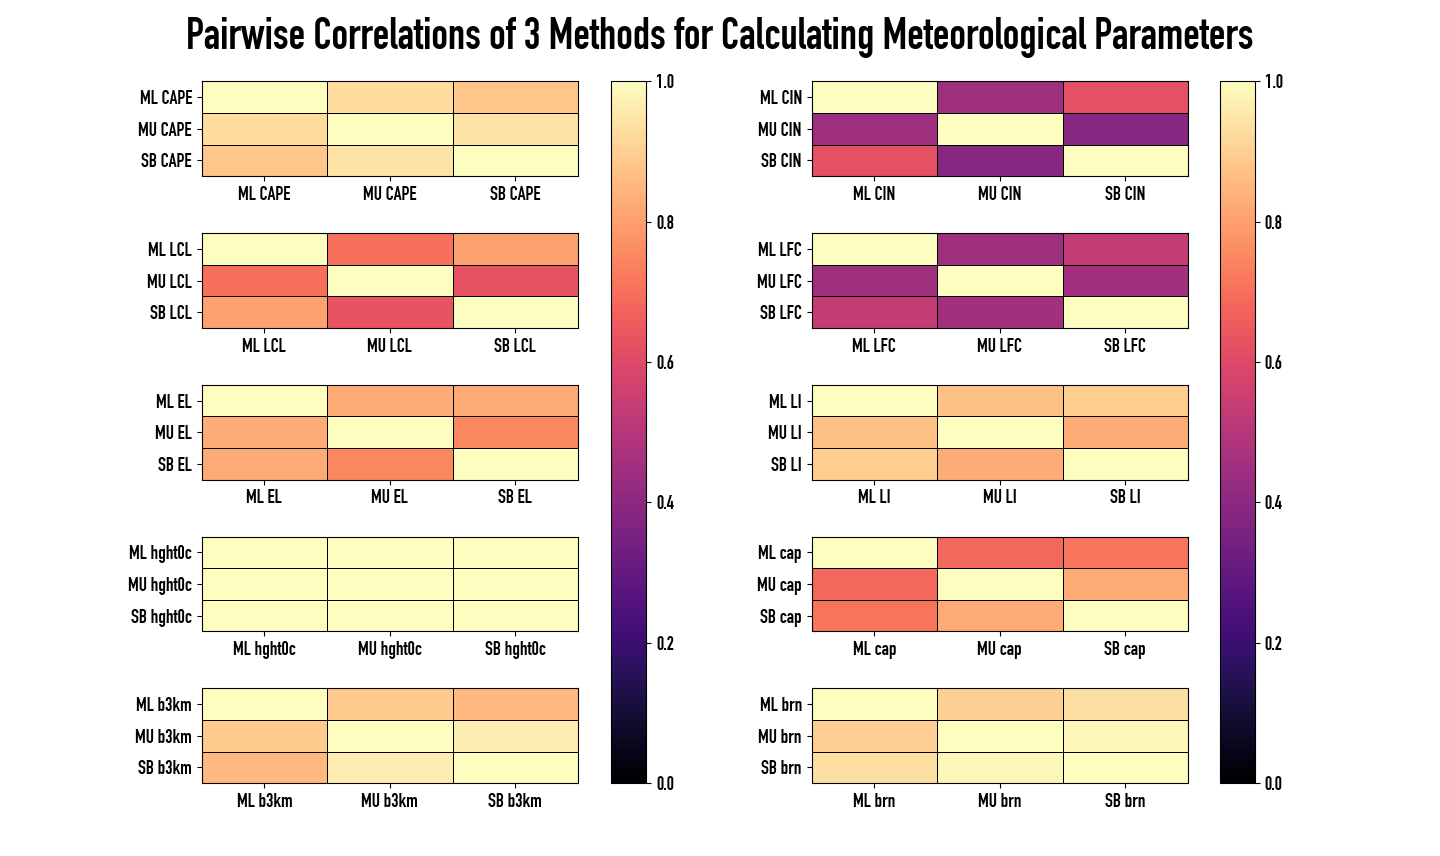
\includegraphics[width=1.15\textwidth, right=19cm]{"plots/big_corrplot.png"} 
\end{figure}

A few of the parameters differ greatly by calculation method; In the most extreme cases (CIN, LFC), MU and ML had a correlation of roughly .4, which is low enough to consider them very different measures. As a result, research was done into which method would yield most accurate results for modeling purposes. While the meteorological field is currently unable to provide conclusive evidence for one method's superiority, it is mentioned in the NOAA Storm Prediction Center source above that ML can produce slightly more accurate predictions of late afternoon cloud base heights. As the severe hail events at the center of our research are exclusively created by thunderstorms (which are most common in the afternoon, when warm and moist air is most often present), it is our opinion that employing the ML parameters in our subsequent visualizations and models will be marginally more effective than the others. Accordingly, any unspecified reference to one of the 11 variables in question will refer to the ML version.

There is, of course, a possibility of revising the data during the modeling phase if results are unsatisfactory, which may include bringing in other parameters that can be found with the same sounding profile described in the Data Description, using the SB or MU methods in addition to ML if they do not excessively increase computational complexity, or even finding a source of higher-resolution sounding profiles (3 hour intervals instead of 6, for example.)

\clearpage

\subsection{Handling Missing Values}

The data contains 20,920 missing values; 2708 in LFC, 2069 in EFF INFLOW, and 16143 in CAP. Due to the entirely continuous nature of the data, we deemed it acceptable to apply KNN (K-Nearest Neighbors) Imputation over the data. In our case, we do this by calculating the weighted mean (the more similar points are, the more they factor into the mean) of the 5 most similar points for any entry with a missing value. This weighted mean is entered as the new value in place of any missing value. The process has the quality of maintaining both mean and variance between the pre- and post-transformation data, which we visualize below with a scatterplot. Each axis represents either the original or imputed data, and each red point represents the square root of mean or standard deviation for one of the three variables that were modified by KNN Imputation. The blue line has a slope of 1, so any points that fall on the blue line represent variables that maintain their distribution after KNN Imputation.

\begin{figure}[H]
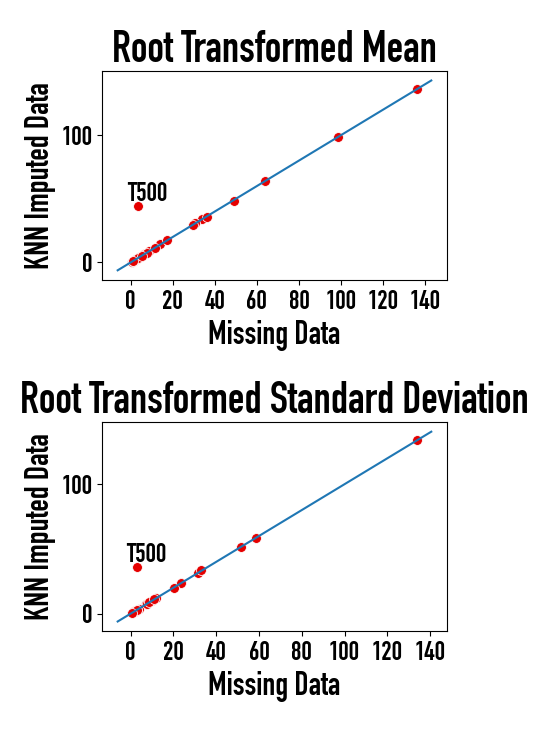
\includegraphics[width=0.5\textwidth, center=8.5cm]{"plots/imputation_plot.png"} 
\end{figure}

\newpage

We can be sure no others variables changed during the application of KNN Imputation over the data, so our only variables of concern are the three we did modify. To be sure that the information they contain was not transformed, we test both their mean and standard deviations before and after transformation; they are nearly identical, so we can confidently conclude that we successfully imputed missing data without modifying the underlying distribution.

\subsection{Exploratory Data Analysis}

We can begin our analysis with the most simple plot of all; we can observe how HAIL SIZE IN, our target variable, is distributed with just two histograms each with different y-axes (linear and log scales). Of interest in these plots is infrequently a report of very large hailstones is received; the right tail is almost invisible on our normal histogram. This means that any modeling we perform will have to be trained more on the infrequent data, as that is the very behavior we are looking to predict due to large hail's ability to cause significant property damage.

\begin{figure}[H]
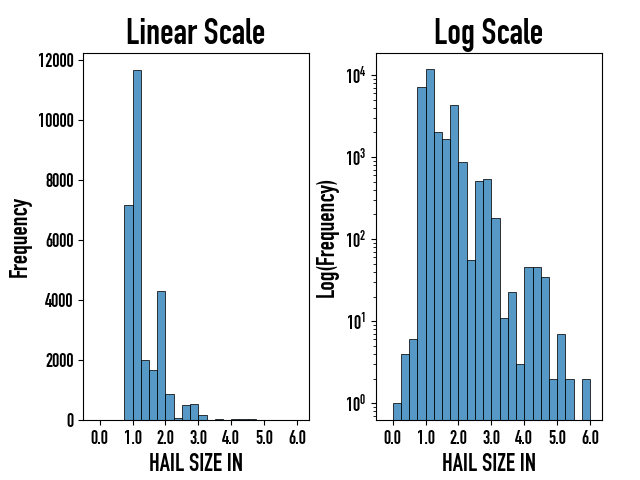
\includegraphics[width=0.6\textwidth, center=8.5cm]{"plots/hail_hist.png"} 
\end{figure}

With so many samples from a naturally occuring phenomenon, it is reasonable to expect our HAIL SIZE IN variable to follow a preexisting distribution. The visual test for this is the QQ Plot, in which the theoretical quantiles of a statistical distribution are compared to actual quantiles found in our sample data. If a line can be draw straight through and capture the direction of the points, then we say that our variable is drawn from the theoretical distribution we used for the QQ Plot. To find our theoretical distribution, we simply run it HAIL SIZE IN through a library that iteratively test dozens of distributions and automatically determine which one best fits our data according to Sum of Squared Error. We found that a generalized normal distribution with shape of 0.48, mean of 1, and SD of 0.028.

\begin{figure}[H]
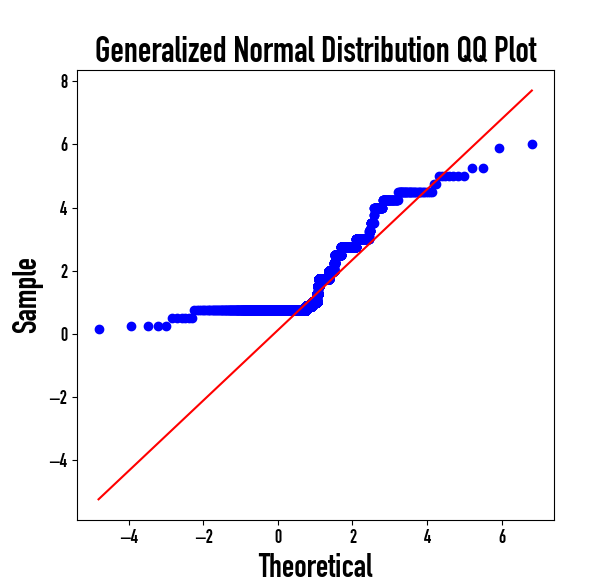
\includegraphics[width=0.6\textwidth, center=8.5cm]{"plots/qq_plot.png"} 
\end{figure}

Upon generating the QQ Plot, it becomes clear that there is a fundamental problem with our data if this is the best distribution we can picture it against. This can be explained, at least in part, by the very nature of the data we collected; NOAA only collects reports of hail that range from 0.75" upwards, which is why we see only a few points in our sample quantile below this on the QQ Plot. Of course, filtering out what might be a significant portion of the actual data is likely to have prevented us from finding the true distribution the data was drawn from, but this is just one of the facts we must handle when dealing with real data, which may be fundamentally biased.

To find patterns in more than just a few variables, we can turn to a correlation plot. This shows pairwise correlation for every variable in the data, so it can be expected to reveal any linear trends between parameters. A few such trends can be noted: CAPE and SRH have almost no correlation, which is fortunate; CAPE represents energy potential for a storm, and SRH measures twisting forces in storms. When both variables are high, they generally provides a good condition for large thunderstorms to occur, so the fact that they must occur independently is beneficial for those who are not partial to frequent large thunderstorms.

One abnormality you might spot is LI's (Lifted Index) strong negative correlation with many of the other parameters, represented by a dark purple line through the chart. This is seems odd, but the explanation is quite simple; it is the only parameter that is always negative as a result of how it is measured, and it is most related to CAPE, so it makes sense for it to have a very strong negative correlation with anything else that is similar to CAPE. 

\begin{figure}[H]
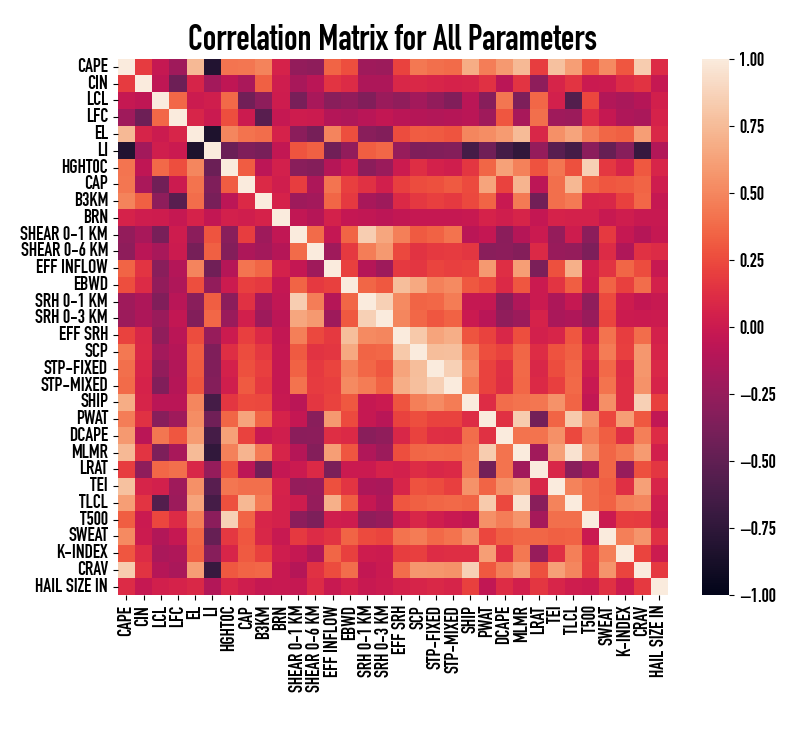
\includegraphics[width=0.5\textwidth, center=8.5cm]{"plots/all_corrs.png"} 
\end{figure}

To briefly cover a few of the many remaining insights this chart has to offer, we have to understand the breakdown of these variables. 1-14 are all metrics calculated from just the original sounding profile we found, but after that, many of the parameters are actually composites, or (mostly) linear compositions of the other parameters that, when combined, form a more useful measure. This is why so much of the correlation plot has high correlation (light colors); many of the parameters we have are based on one another, so it is to be expected that they should increase or decrease along with the others. It may seem like having the composite variables would be unnecessary then, but there are two primary reasons to keep them: first, a few of them contain information not held in our parameters 1-14, and modeling is entirely focused on analyzing as much quality information as possible. Second, depending on the type dimensionality reduction applied, it is very likely that we will be dealing with very few dimensions during our modeling phase, and having a few somewhat redundant variables form our components would not be a detriment to the model; rather, it just might allow for more representative ways to combine the data.

Finally, turn your attention to the bottom row or rightmost column of the plot, where HAIL SIZE IN is located. The row is by far the most uniform in color, with low correlation across all variables. This is why we are performing our research; if it were linearly correlated with one of our other parameters, then predicting hail size would be trivial. In fact, the highest-correlation parameter to HAIL SIZE IN, which is SHIP, is still not even above a correlation of around 0.2. This is no surprise, however, as SHIP is not actually intended to forecast hail sizes, but rather to classify hail events as likely to produce hail above or below 2". We can see how well it works by sorting the data into two bins around 2" and plotting SHIP's boxplots for each, as below.

\begin{figure}[H]
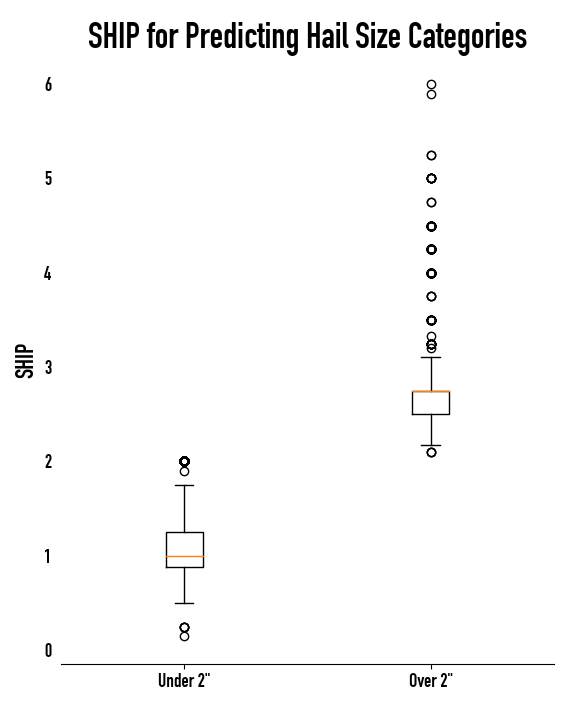
\includegraphics[width=0.5\textwidth, center=8.5cm]{"plots/ship_boxplots.png"} 
\end{figure}

While SHIP appears to work incredibly well at for separating hail sizes into two groups, we are attempting a much trickier task: accurate regression. This will be the primary focus of the next section of the paper, and will build off of many of the concepts and ideas expressed throughout the past two sections.


\bigskip
\bigskip
%----------------------------------------------------------------------------------------
 % Algorithm and Methodology
%----------------------------------------------------------------------------------------


\section{Algorithm and Methodology}

The algorithms used in the experimentation section of this report are simply the ten most popular regression algorithms available for Python, according to the Educative Blog. Most of these are based on linear regression or random forests, but small differences in loss functions or other peculiarities cause them to perform very differently over the data. The simplest of these ten models was ordinary least squares linear regression, which simply fits a line to the data by minimizing residiual errors. While this is a very common approach, it was clear from the low correlation found in the above sections that no linear combination of variables would provide good predictions for Hailstone Size. Therefore, other methods will be used. 

The two most similar models to linear regression are SGD (Stochastic Gradient Descent) Regression and ElasticNet. SGD differs only in the method of minimizing the loss function; rather than using a deterministic approach like Ordinary Least Squares allows, it iteratively decreases a loss function by following a gradient downwards. ElasticNet is actually a particular case of SGD that combines L1 and L2 norms to regularize the function, where SGD only uses one or the other.

The other model I will test variations of is almost identical to ordinary least squares linear regression: Ridge Regression. In short, Ridge Regression attempts to reduce overfitting in the model by adding a bias term while calculating the Residual Sum of Squares for the regression line. This is a classic case of the standard tradeoff in machine learning, bias vs. variance. Here, fit error (bias) is increased at to allow for better extensibility of the model (variance). The two versions of Ridge Regression that I will employ are Bayesian Ridge and Kernel Ridge. Bayesian is similar to regular Ridge Regression more in function than in form; it operates over probabilistic spaces rather than distance, but makes the same tradeoff as Ridge Regression in decreasing variance at the cost of increased bias. While Bayesian Ridge is easy to apply to any dataset for regression, it has the unfortunate downside of having very expensive inference due to the sheer number of probabilites that are calculated and stored for use. Kernel Regression is a hybrid of Ridge Regression that also allows for non-linear combinations of the features to be formed, which may increase accuracy of the model at the expense of higher training time and model complexity. Similar to Kernel Regression is SVR (Support Vector Regression), which is identical but for the cost function employed; while Kernel Ridge uses squared error loss, SVR uses $\epsilon$-insensitive loss, which is exactly what it sounds like; any error less than $\epsilon$ is ignored, leading to very different outcomes than squared loss.

The other four algorithms are all variations on Gradient Boosting and Decision Trees, with varying degrees of complexity. This includes Gradient Boosting, XGBoost, LGBM, and CatBoost. Gradient Boosting is a model similar to Random Forests, but with a few clear advantages: instead of filling out each tree to its full depth, Gradient Boosting relies on many smaller trees (or "weak learners") that are made to minimize the predefined loss function. This allows Gradient Boosting to generally outperform Random Forests, but there are numerous modificiations that can be made to Gradient Boosting to improve it as well. XGBoost (Extreme Gradient Boosting) is a particular implementation of Gradient Boosting that is designed to be both more accurate and more computationally effective than other algorithms. Another modification of standard Gradient Boosting is LGBM (Light Gradient Boosting Model), which adds a combination of other techniques that can reduce computational complexity and increase information gained from small datasets. Finally, CatBoost is an implementation of Gradient Boosting that fundamentally changes how the aforementioned "weak learners" are built. These Gradient Boosting methods are rapidly gaining popularity (largely among those who are tired of hearing Neural Nets mentioned constantly).


\bigskip
\bigskip
%----------------------------------------------------------------------------------------
 % Experiments and Results
%----------------------------------------------------------------------------------------
\section{Experiments and Results}

Some considerations must be made in terms of this project's methodology. First, protecting against overfitting: to avoid this, I will be employing a train-test-validate split of 60-25-15 for the data. To do this, I will first split the data 75-25 after normalization, and set aside the smaller portion for use as the final test set. Then, each of the ten algorithms above will be used in 5-fold cross validation with the default model hyperparameters. My primary accuracy metric will be MAE (Mean Absolute Error), and it is important to note that regression model performance is entirely relative, as there is no class to compare it to or confusion matrix to analyze. By taking the mean of the 5 accuracy scores returned for each algorithm, I will sort the models by their performance. The best 3 models will become my focus, and I will use the trained models to predict Hailstone Size for the held-out remainder of the data. The MAE for each of these three models will determine which algorithm was most effective over this dataset. 

\begin{figure}[H]
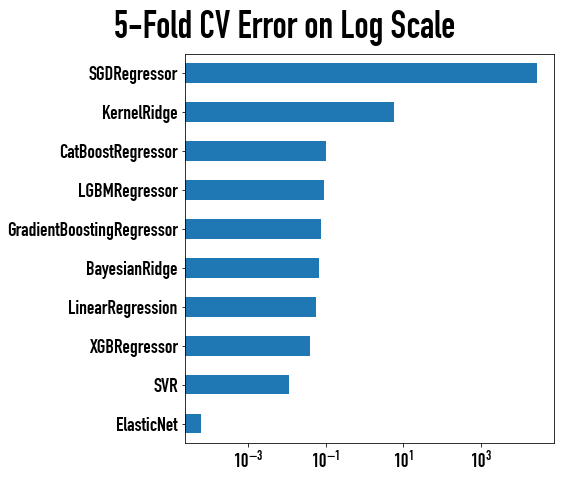
\includegraphics[width=0.5\textwidth, center=8.5cm]{"plots/5-fold.png"} 
\end{figure}

The results of the 5-fold Cross-Validation, shown above, clearly show XGBoost, SVR, and ElasticNet to be the three lowest-error models, but before those are discussed, we have to ask: why is the average error for SGD Regression so incredibly high? Coming in around 26,000, it is orders of magnitude greater than most of our other models. The best explanation I can provide for this comes from the actual definition of SGD. SGD works by randomly sampling the data and calculating the gradient of those samples only, then moving the parameters in whichever direction minimizes the loss function. This, however, also explains why it has such high potential for error; if the data is not well-suited for random sampling or the samples taken do not represent the data well, then SGD is capable of failing massively when the model produced is actually evaluated. This is corroborated by observing the errors for each fold; the absolute errors produced for this run of SGD range from 0.05 to approximately 140,000. This tells us that SGD may be capable of producing good results, but an optimized version of it (like ElasticNet) that is more consistent will almost certainly be a better choice for final models.

Now that we have resolved why SGD has been so ineffective, we can analysze the efficacy of the 3 models that were found to have the lowest error. The trained models from the 5-fold CV were returned at the end and saved, so we simply have to use each of the 5 instances of the 3 models to perform inference on the held-out quarter of the data from earlier. By doing this, and using the Mean Absolute Error method mentioned above, and averaging the errors for each group of 5 trained models, we find the following errors. 

\begin{figure}[H]
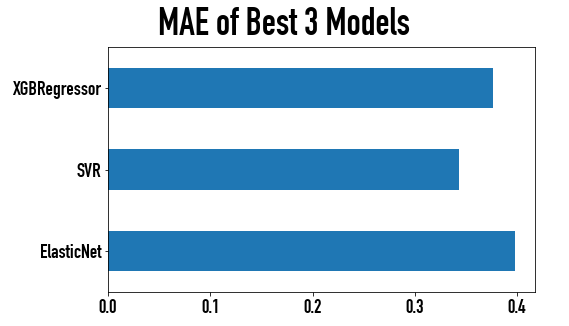
\includegraphics[width=0.5\textwidth, center=8.5cm]{"plots/3_mae.png"} 
\end{figure}

Somewhat surprisingly (given its higher error), the SVR (Support Vector for Regression) performed significantly better than the other two models, yielding mean absolute errors around 0.34". This means that, given all of the variables used to train the model, it could predict hailstone sizes to within a third of an inch, on average. The other models were closer to 0.4", so for our purposes, we would probably avoid them in favor of SVR.

\bigskip
\bigskip
%----------------------------------------------------------------------------------------
 % Summary and Conclusions
%----------------------------------------------------------------------------------------
\section{Summary and Conclusions}

This report was produced with the intention of developing a better method to predict the size of hailstone events prior to their occurence. The data was collected after the events, but the best model found (SVR) suggests that hailstone sizes could be predicted to within an accuracy of one-third of an inch, on average. Further study might involve more extensive model selection, the usage of Neural Networks for regression, hyperparameter optimization on whichever algorithms already produce the best results, or even development of a pipeline to automatically collect broader data (for example, if the data was converted to time-series by adding date as a variable, seasonal trends could contain information not available in this study). As it stands, the limited body of research in hailstone modeling seems ripe for improvement as Machine Learning algorithms undergo a Renaissance of development and improvement, but such advanced algorithms were deemed to be outside the purview or capacity of this study.

\bigskip
\bigskip
\bigskip



\phantomsection
\section*{Acknowledgments} % The \section*{} command stops section numbering
Cody Kirkpatrick, Ph.D. \newline
Hasan Kurban, Ph.D \newline
Anand, A. (n.d.). Scikit-learn cheat sheet: Methods for classification \and; regression. Educative. Retrieved May 3, 2022, from \url{https://www.educative.io/blog/scikit-learn-cheat-sheet-classification-regression-methods} \newline
Learn: Machine learning in python - scikit-learn 0.16.1 documentation. scikit. (n.d.). Retrieved May 3, 2022, from \url{https://scikit-learn.org/} \newline
Megna, M. (2021, June 16). Hail Damage Home Insurance claims: What you need to know. Insurance.com. Retrieved May 3, 2022, from \url{https://www.insurance.com/coverage/home-hail-damage-insurance-claims#:~:text=hail\%5C\%20damage\%5C\%20insurance-,Average\%5C\%20insurance\%5C\%20payout\%5C\%20for\%5C\%20hail\%5C\%20damage,may\%5C\%20be\%5C\%20higher\%5C\%20or\%5C\%20lower\%22} \newline
Schrater, P. (n.d.). Regression part II - vision labs. Regression II. Retrieved May 3, 2022, from \url{http://vision.psych.umn.edu/users/schrater/schrater_lab/courses/PattRecog09/RegressionII.pdf} \newline
\addcontentsline{toc}{section}{Acknowledgments} % Adds this section to the table of contents



%----------------------------------------------------------------------------------------
%	REFERENCE LIST
%----------------------------------------------------------------------------------------
\phantomsection
\bibliographystyle{srt}


%----------------------------------------------------------------------------------------

\end{document}